% !TEX root = ../thuthesis-main.tex

\chapter{实验结果}

本章展示实验结果与分析。首先介绍数据集的构建过程与统计特征；随后通过对照实验验证本文评价指标的有效性；接着分别报告两阶段模型的定量评估结果与错误模式分析；最后报告强化学习阶段的实验结果。


\section{数据集构建与分析}

本节介绍训练数据集的构建过程与统计特征。

\subsection{数据规模}

本文的数据源为公开数据集Verilog\_GitHub\inlinecite{thakur2024verigen}，该数据集从GitHub公开仓库中收集了108{,}971个Verilog源文件。经过第~\ref{chap:method}~章所述的多层级筛选流程后，最终保留5{,}847个有效模块用于数据合成。

从108{,}971个原始文件到最终5{,}847个有效样本，整体保留率约为5.4\%。大量文件在筛选过程中被排除，主要原因包括：Icarus Verilog编译错误（语法不合规或使用了不支持的语言特性）、仿真运行失败（如死循环导致超时、信号未正确初始化等）、依赖外部文件（\texttt{`include}指令、\texttt{\$readmemh}系统调用）导致无法独立仿真、包含多模块定义、属于工艺库标准单元而非可综合RTL设计，以及仿真产出的图像尺寸或信号数量超出合理范围等。

\subsection{信号数量分布}

每个样本的信号数量反映了对应电路模块的端口复杂度，Verilog源代码的长度则反映了模块的逻辑复杂度。图~\ref{fig:dataset-dist}展示了数据集中样本的信号数量与代码长度分布。

\begin{figure}[htbp]
  \centering
  \begin{minipage}{\textwidth}
    \centering
    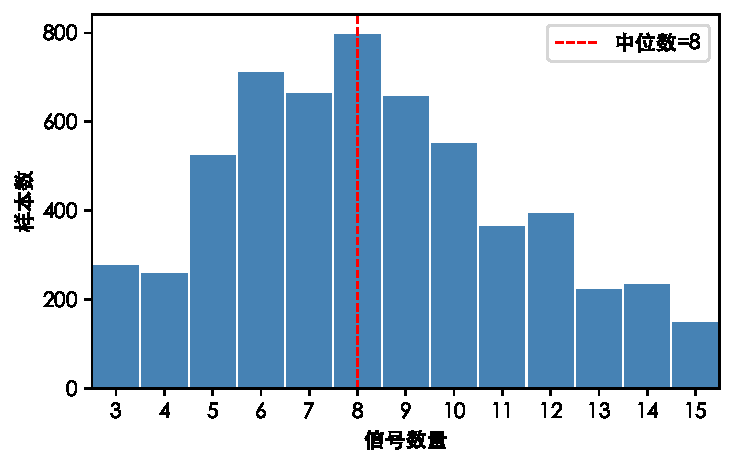
\includegraphics[width=0.65\textwidth]{figures/signal_count_dist.pdf}
    \centerline{（a）信号数量分布}
  \end{minipage}
  \vspace{0.3em}
  \begin{minipage}{\textwidth}
    \centering
    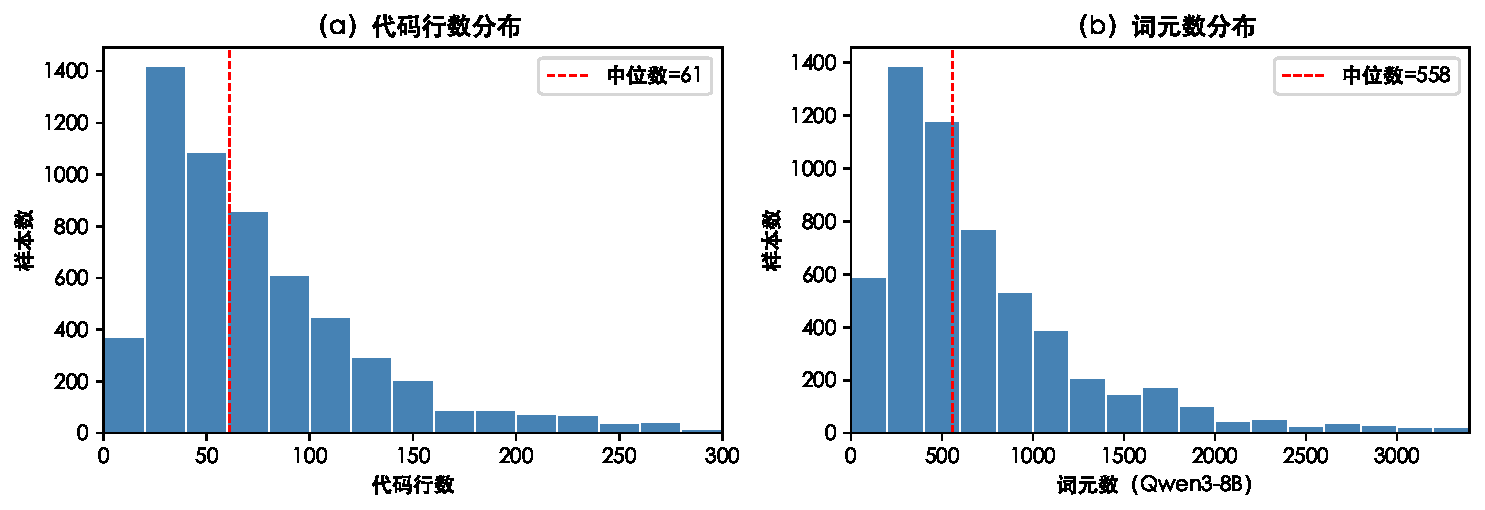
\includegraphics[width=\textwidth]{figures/code_length_dist.pdf}
    \centerline{（b）Verilog代码长度分布}
  \end{minipage}
  \caption{数据集样本的信号数量与代码长度分布}
  \label{fig:dataset-dist}
\end{figure}

信号数量主要集中在5至10个之间，占比约67\%，中位数为8个信号。这一分布覆盖了从简单门电路（3--4个端口）到中等复杂度模块（13--15个端口）的广泛范围，为模型训练提供了不同复杂度层次的样本。代码行数（去除注释与空行后）的中位数为61行，均值为89行，主要集中在21至120行之间（约75\%）。词元数的中位数为350，均值为536，主要集中在101至700之间（约78\%）。两个维度均呈现右偏分布，少数大型模块（如总线协议控制器、多级流水线运算单元）的代码长度显著高于平均水平。整体而言，数据集中的模块以中等规模为主，兼顾了训练效率与逻辑复杂度的多样性。

\subsection{数据划分}

经过第~\ref{chap:method}~章所述的防泄漏划分策略，5{,}847个样本被划分为训练集5{,}730个与测试集117个。两个阶段的训练与评估均使用相同的划分方案。

\subsection{模块功能多样性}

为评估数据集覆盖的电路功能类型，本文基于模块名称的自动化分段匹配对5{,}847个模块进行了功能分类。具体方法为：首先从测试平台文件中提取被测模块（DUT）的Verilog模块名；然后将模块名按下划线与驼峰命名边界拆分为词段序列（例如\texttt{axi\_protocol\_converter\_v2\_1\_b2s\_simple\_fifo}拆分为\texttt{[axi, protocol, converter, ..., simple, fifo]}）；接着将每个词段与预定义的关键词-类别映射表进行匹配，该映射表的关键词来源于对全部2{,}362个不同模块名的词段频率统计，选取出现频率最高的功能性词段（如\texttt{fifo}、\texttt{fsm}、\texttt{counter}、\texttt{mux}等）作为类别关键词。关键词分为两个层级：功能关键词（描述电路功能，如\texttt{fifo}、\texttt{counter}）与上下文关键词（描述总线接口，如\texttt{axi}、\texttt{spi}、\texttt{uart}）。分类规则为：当模块名中恰好出现一个功能关键词时，归入对应类别；仅出现上下文关键词时，归入通信控制器；出现多个不同类别的功能关键词时，为避免歧义，保守地归入“其他”类别。分类结果如表~\ref{tab:module-category}所示。

\begin{table}[htbp]
  \centering
  \caption{数据集模块功能分类统计}
  \label{tab:module-category}
  \begin{tabular}{lrr}
    \toprule
    功能类别 & 模块数 & 占比 \\
    \midrule
    通信控制器 & 540 & 9.2\% \\
    FIFO & 350 & 6.0\% \\
    时钟与同步 & 258 & 4.4\% \\
    状态机 & 197 & 3.4\% \\
    多路选择器 & 170 & 2.9\% \\
    算术逻辑单元 & 166 & 2.8\% \\
    存储器 & 161 & 2.8\% \\
    定时器 & 129 & 2.2\% \\
    计数器 & 125 & 2.1\% \\
    GPIO与外设 & 76 & 1.3\% \\
    编解码器 & 50 & 0.9\% \\
    CRC与校验 & 47 & 0.8\% \\
    寄存器堆 & 36 & 0.6\% \\
    移位寄存器 & 35 & 0.6\% \\
    其他 & 3{,}507 & 60.0\% \\
    \bottomrule
  \end{tabular}
\end{table}

基于模块名的分类方法具有高精确度——每个分类结果均可直接从模块名验证，且分类规则不涉及任何启发式歧义消解。为评估分类的可靠性，本文将模块名分类结果与LLM生成测试平台时输出的模块功能描述文本进行交叉验证：对每个被分类的模块，检查其LLM分析文本中是否包含与分类类别相关的功能关键词。交叉验证结果显示，95.6\%的分类结果被LLM分析文本所确认，其中6个类别的确认率达到100\%，表明基于模块名的分类具有较高的可靠性。未被确认的4.4\%主要来自LLM分析文本未显式提及功能关键词的情况（如仅列出端口表而未描述模块功能），而非实际的分类错误。

约40\%的模块被成功分类。通信控制器占比最高（9.2\%），主要来源于AXI、SPI、UART、PCIe等总线接口与串行通信接口的子模块；FIFO（6.0\%）与时钟同步电路（4.4\%）紧随其后，反映了数据缓冲与跨时钟域同步在数字设计中的普遍性。算术逻辑单元（2.8\%）包含整数运算器与浮点运算子模块，存储器（2.8\%）涵盖了单端口与双端口RAM、ROM、缓存等。状态机、多路选择器、定时器、计数器等常见功能模块均有分布。“其他”类别（60.0\%）的构成较为多样，主要包括以下几类：项目专用名称或缩写无法自动识别功能的模块（如\texttt{csrbrg}、\texttt{ablk}等），含有通用功能词但语义过于宽泛的模块（如各类\texttt{controller}、\texttt{control}模块），FPGA IP核中的数据通路适配子模块（如总线宽度转换器\texttt{DecWidthConverter}、协议适配器\texttt{MM\_to\_ST\_Adapter}等），VGA显示控制器、边沿检测器等占比较小的功能类别，以及少量多关键词冲突而保守归入“其他”的模块。整体而言，已分类模块涵盖了从基础逻辑单元到中等复杂度时序电路的广泛功能类型，表明数据集具备良好的功能多样性。

\subsection{时序图样本示例与激励方案对比}

本节通过具体样本展示两种测试平台生成方案产生的时序图差异，以直观说明激励质量对训练数据的影响。

\textbf{状态机对比。}%
图~\ref{fig:fsm-comparison}展示了一个多状态FSM模块（\texttt{FsmExample}）在两种激励下的时序图。该模块以两个输入信号\texttt{a}、\texttt{b}驱动状态转移，通过3位输出\texttt{dout}指示当前状态。随机激励方案中，gentbvlog正确识别了时钟信号并生成了周期性驱动，复位信号\texttt{rst\_n}也恰好经历了正确的置位-释放序列，状态机在复位后正常运行。然而，输入信号\texttt{a}与\texttt{b}的随机组合缺乏功能覆盖性——在整个仿真过程中仅产生了4种可能输入组合中的2种，导致\texttt{dout}只在状态1与状态2之间来回切换，状态3从未被触发。LLM激励方案在分析模块的状态转移逻辑后，设计了覆盖性的输入序列：先完成规范的复位初始化，随后系统地组合\texttt{a}与\texttt{b}的不同取值以覆盖全部转移路径，输出\texttt{dout}在20个时钟周期内循环经过全部状态值（$1 \to 2 \to 1 \to 3 \to 1 \to 2 \to 3 \to 2 \to \ldots$），完整展示了状态机的转移行为。

\begin{figure}[htbp]
  \centering
  \begin{minipage}{\textwidth}
    \centering
    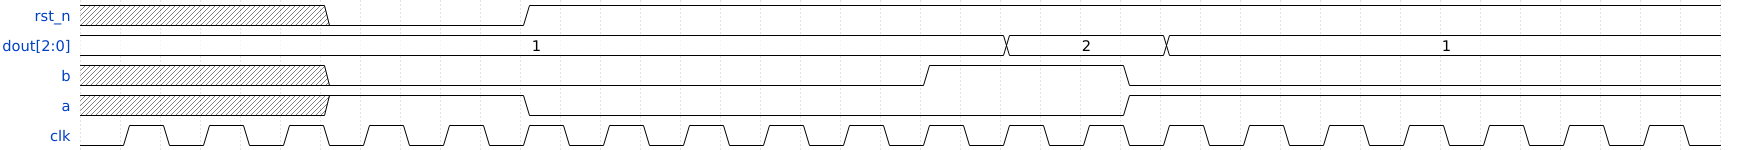
\includegraphics[width=\textwidth]{figures/samples/fsm_new.png}
    \centerline{（a）随机激励}
  \end{minipage}
  \vspace{0.5em}
  \begin{minipage}{\textwidth}
    \centering
    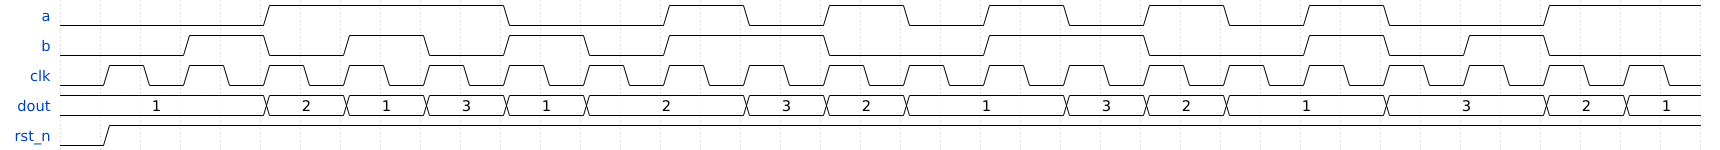
\includegraphics[width=\textwidth]{figures/samples/fsm_new_llm.png}
    \centerline{（b）LLM激励}
  \end{minipage}
  \caption{同一状态机模块在两种激励方案下的时序图对比}
  \label{fig:fsm-comparison}
\end{figure}

\textbf{FIFO对比。}%
图~\ref{fig:fifo-comparison}展示了同一8位FIFO模块在两种激励下的时序图。两种方案均使用了正确的周期性时钟，差异完全来自激励策略。随机激励方案将复位、入队使能（\texttt{push}）、出队使能（\texttt{pop}）与8位数据输入打包为一个11位数组，由\texttt{\$random}统一驱动。产生的时序图中，复位信号在仿真初期长时间保持有效，使FIFO大部分时间处于复位状态；入队与出队使能信号的跳变缺乏协调，数据输入端口呈现无意义的随机十六进制值（\texttt{A4}、\texttt{D0}、\texttt{C1}等），\texttt{full}与\texttt{empty}标志始终不变，数据输出\texttt{data\_out}几乎为常量，FIFO的核心功能未能被激活。LLM激励方案在分析模块功能后设计了结构化的操作序列：先短暂断言复位信号完成初始化，随后进入入队阶段依次写入具有工程辨识度的测试向量（\texttt{0xAA}、\texttt{0x55}、\texttt{0xFF}、\texttt{0x00}、\texttt{0x33}、\texttt{0xCC}等），当FIFO写满时\texttt{full}标志正确置位；接着进入出队阶段，\texttt{data\_out}按先入先出顺序依次输出此前写入的数据，\texttt{empty}标志在FIFO清空时正确置位。两个标志位的状态翻转清晰可见，完整展示了FIFO的缓冲与流控行为。

\begin{figure}[htbp]
  \centering
  \begin{minipage}{\textwidth}
    \centering
    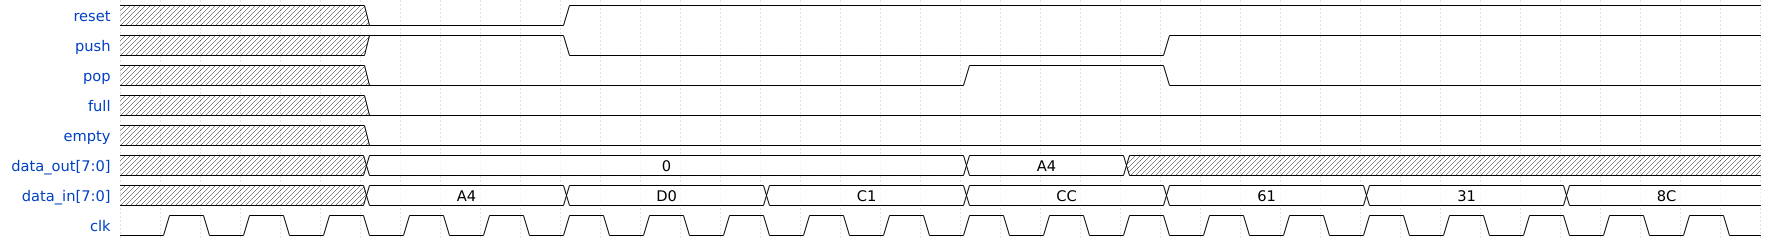
\includegraphics[width=\textwidth]{figures/samples/fifo2.png}
    \centerline{（a）随机激励}
  \end{minipage}
  \vspace{0.5em}
  \begin{minipage}{\textwidth}
    \centering
    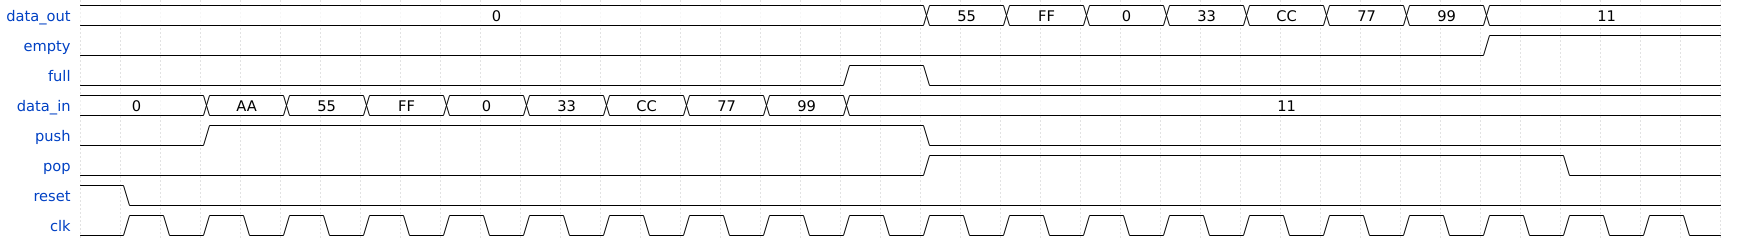
\includegraphics[width=\textwidth]{figures/samples/fifo2_llm.png}
    \centerline{（b）LLM激励}
  \end{minipage}
  \caption{同一FIFO模块在两种激励方案下的时序图对比}
  \label{fig:fifo-comparison}
\end{figure}

上述两组对比揭示了随机激励方案的核心局限：缺乏功能语义的激励序列使得模块的关键行为模式（状态遍历、标志位翻转等）无法在仿真中被充分激活，产生的时序图对模型训练贡献有限。LLM激励方案通过理解模块功能语义生成有目的的激励，使时序图能够充分展示模块的各种工作状态，为模型提供更具区分度的训练样本。同时，高覆盖率的激励序列也使得第二阶段的仿真对拍评估更加可靠——随机激励下大量输出信号保持常量，即使生成代码存在功能错误也可能碰巧通过对拍；而LLM激励充分激活了模块的各种工作状态，使对拍结果能够更有效地检测生成代码的功能缺陷。

图~\ref{fig:sample-diversity}展示了数据集中不同功能类别模块的时序图样本，体现了数据集在信号类型与波形模式上的多样性。超前进位加法器模块以纯组合逻辑为主，无时钟信号，输入\texttt{a}、\texttt{b}与进位\texttt{cin}驱动求和输出\texttt{s}与进位输出\texttt{cout}，波形呈现密集的数据标签跳变；UART控制器模块展示了串行通信接口的典型交互模式，包含写数据\texttt{wr}、发送请求\texttt{trx\_req}、串行输出\texttt{trx}与应答\texttt{trx\_ack}等握手信号；RAM模块实现了基于双端口存储器的FIFO缓冲功能，时序图中可见写使能\texttt{wr\_en}与读使能\texttt{rd\_en}交替驱动数据的入队与出队，\texttt{full}、\texttt{empty}及其预警标志\texttt{a\_full}、\texttt{a\_empty}随缓冲区状态翻转，完整展示了FIFO的流控行为。

\begin{figure}[htbp]
  \centering
  \begin{minipage}{\textwidth}
    \centering
    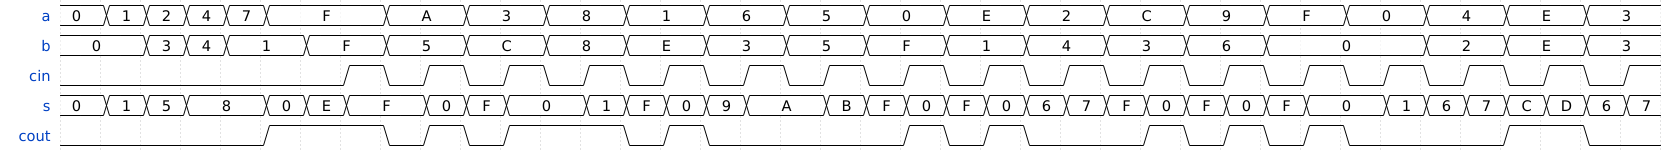
\includegraphics[width=\textwidth]{figures/samples/adder.png}
    \centerline{（a）超前进位加法器（\texttt{LookAheadAdder}）}
  \end{minipage}
  \vspace{0.5em}
  \begin{minipage}{\textwidth}
    \centering
    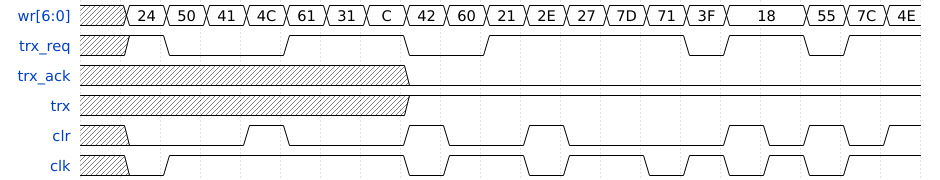
\includegraphics[width=\textwidth]{figures/samples/uart.png}
    \centerline{（b）UART控制器（\texttt{uart\_ctrl}）}
  \end{minipage}
  \vspace{0.5em}
  \begin{minipage}{\textwidth}
    \centering
    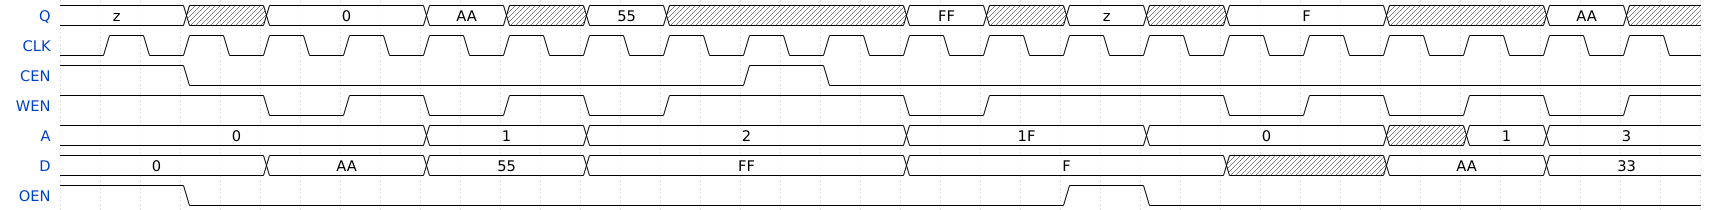
\includegraphics[width=\textwidth]{figures/samples/ram.png}
    \centerline{（c）RAM存储器（\texttt{ram}）}
  \end{minipage}
  \caption{数据集中不同功能类别的时序图样本}
  \label{fig:sample-diversity}
\end{figure}


\section{评价指标有效性分析}

第~\ref{sec:metrics}~节提出了面向时序图结构化表示的专用评价指标。为验证该指标相比传统文本相似度指标的有效性，本节通过一组对照实验进行对比分析。对照基线选用两种广泛使用的文本相似度指标：Levenshtein比率\inlinecite{levenshtein1966binary}（将标准答案与预测结果的WaveJSON序列化文本进行字符级编辑距离比较）与BLEU\inlinecite{papineni2002bleu}（将WaveJSON序列化文本按词元分割后计算$n$-gram精确率）。

本文选取五个具有代表性的评估场景，分别对应时序图解析中常见的差异类型，涵盖了文本相似度“虚低”（语义一致但文本不同）与“虚高”（语义不同但文本相似）两类典型失效模式。各场景的评分对比结果如表~\ref{tab:metric-comparison}所示。

\begin{table}[htbp]
  \centering
  \caption{传统文本相似度指标与本文评价指标的对比}
  \label{tab:metric-comparison}
  \begin{tabular}{clcccccc}
    \toprule
    \multirow{2}{*}{编号} & \multirow{2}{*}{场景} & \multirow{2}{*}{Levenshtein} & \multirow{2}{*}{BLEU} & \multicolumn{3}{c}{本文指标} \\
    \cmidrule(lr){5-7}
     &  &  &  & P & R & F1 \\
    \midrule
    1 & 信号顺序置换 & 0.912 & 0.952 & 1.000 & 1.000 & 1.000 \\
    2 & 保持符号等价 & 0.939 & 0.845 & 1.000 & 1.000 & 1.000 \\
    3a & 少量数据标签错误（1/4） & 0.991 & 0.928 & 0.875 & 0.875 & 0.875 \\
    3b & 大量数据标签错误（4/4） & 0.966 & 0.777 & 0.500 & 0.500 & 0.500 \\
    4 & 信号缺失（4缺1） & 0.897 & 0.801 & 1.000 & 0.750 & 0.857 \\
    \bottomrule
  \end{tabular}
\end{table}

\textbf{场景1：信号顺序置换。}如图~\ref{fig:metric-s1}所示，预测结果包含与标准答案完全相同的三个信号（时钟、输入、输出），渲染出的时序图在视觉上完全一致，仅信号在WaveJSON数组中的排列顺序不同。由于信号排列顺序仅影响渲染时的纵向位置，不改变任何时序语义，因此应获得满分。Levenshtein比率因数组元素位置变化产生了8.8\%的扣分，BLEU虽受影响较小（0.952）但仍未给出满分，而本文指标通过基于信号名的匹配策略正确给出1.0的满分。

\begin{figure}[htbp]
  \centering
  \begin{minipage}{0.32\textwidth}
    \centering
    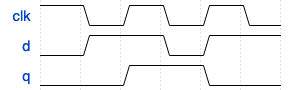
\includegraphics[width=\textwidth]{figures/metrics/s1_gt.png}
    \centerline{标准答案}
  \end{minipage}
  \hspace{2em}
  \begin{minipage}{0.32\textwidth}
    \centering
    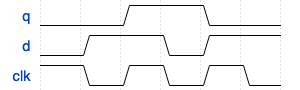
\includegraphics[width=\textwidth]{figures/metrics/s1_pred.png}
    \centerline{预测结果}
  \end{minipage}
  \caption{场景1：信号顺序置换（语义一致，仅纵向排列不同）}
  \label{fig:metric-s1}
\end{figure}

\textbf{场景2：保持符号等价。}如图~\ref{fig:metric-s2}所示，标准答案与预测结果描述的信号行为完全相同，差异仅在于WaveJSON的书写方式：标准答案使用保持符号（\texttt{.}）表示信号在后续时钟周期中延续前一周期的电平（如\texttt{0..1..}表示低电平持续三拍后高电平持续三拍），预测结果则逐周期显式写出电平值（如\texttt{000111}）。两种写法的语义完全等价，但文本差异显著。Levenshtein比率产生了6.1\%的扣分，BLEU的扣分更为严重（0.845），而本文指标在评分前将保持符号展开为实际电平值后进行比较，正确给出满分。

\begin{figure}[htbp]
  \centering
  \begin{minipage}{0.32\textwidth}
    \centering
    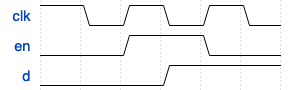
\includegraphics[width=\textwidth]{figures/metrics/s2_gt.png}
  \end{minipage}
  \caption{场景2：保持符号等价（\texttt{0..1..} vs \texttt{000111}，渲染后视觉一致）}
  \label{fig:metric-s2}
\end{figure}

\textbf{场景3：数据标签错误。}如图~\ref{fig:metric-s3}所示，此场景展示指标对语义错误严重程度的区分能力。标准答案包含一个4拍计数器信号，数据标签依次为\texttt{0}、\texttt{1}、\texttt{2}、\texttt{3}。场景3a中仅最后一个标签错误（\texttt{3}$\to$\texttt{4}），场景3b中全部四个标签均错误。从渲染的时序图可以直观看出两种错误的严重程度差异显著。然而Levenshtein比率在两种情况下的得分分别为0.991与0.966，差异仅为0.025；BLEU分别为0.928与0.777，差异为0.151，区分能力优于Levenshtein但仍不充分。而本文指标的F1分数分别为0.875与0.500，差异达到0.375，准确反映了错误从局部到全局的严重程度变化。

\begin{figure}[htbp]
  \centering
  \begin{minipage}{0.32\textwidth}
    \centering
    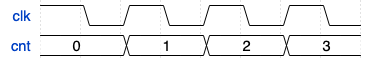
\includegraphics[width=\textwidth]{figures/metrics/s3_gt.png}
    \centerline{标准答案}
  \end{minipage}
  \hfill
  \begin{minipage}{0.32\textwidth}
    \centering
    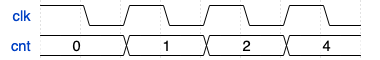
\includegraphics[width=\textwidth]{figures/metrics/s3a_pred.png}
    \centerline{场景3a（1/4错误）}
  \end{minipage}
  \hfill
  \begin{minipage}{0.32\textwidth}
    \centering
    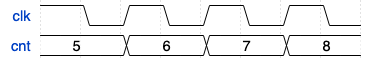
\includegraphics[width=\textwidth]{figures/metrics/s3b_pred.png}
    \centerline{场景3b（4/4错误）}
  \end{minipage}
  \caption{场景3：数据标签错误（标签\texttt{3}$\to$\texttt{4} vs 全部替换）}
  \label{fig:metric-s3}
\end{figure}

\textbf{场景4：信号缺失。}如图~\ref{fig:metric-s4}所示，预测结果遗漏了标准答案中四个信号之一（信号\texttt{b}缺失）。Levenshtein比率给出0.897，BLEU给出0.801，均未能充分反映信息缺失的严重性。本文指标的F1为0.857，其中精确率（Precision）为1.000（预测的信号全部正确），召回率（Recall）为0.750（标准答案中有25\%的信号未被识别）。这一精确率与召回率的分解提供了比单一相似度数值更丰富的诊断信息，有助于分析模型的错误模式——是倾向于“少预测”（召回率低）还是“乱预测”（精确率低）。

\begin{figure}[htbp]
  \centering
  \begin{minipage}{0.32\textwidth}
    \centering
    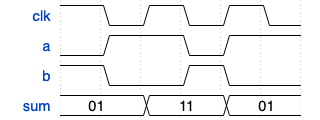
\includegraphics[width=\textwidth]{figures/metrics/s4_gt.png}
    \centerline{标准答案（4个信号）}
  \end{minipage}
  \hspace{2em}
  \begin{minipage}{0.32\textwidth}
    \centering
    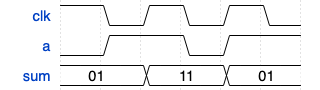
\includegraphics[width=\textwidth]{figures/metrics/s4_pred.png}
    \centerline{预测结果（缺失信号\texttt{b}）}
  \end{minipage}
  \caption{场景4：信号缺失（信号\texttt{b}被遗漏）}
  \label{fig:metric-s4}
\end{figure}

综合以上分析，Levenshtein比率与BLEU等传统文本相似度指标存在两类系统性偏差：对语义无关的文本差异（信号顺序、表示风格）产生不必要的惩罚（场景1、2），同时对语义关键的内容错误（数据标签、信号缺失）缺乏足够的敏感度（场景3、4）。本文设计的评价指标通过信号级匹配、保持符号展开与精确率-召回率分解，在两个方向上均给出了更符合语义正确性的评分。


\section{第一阶段实验结果}

本节报告第一阶段（时序图图像到WaveJSON）有监督微调模型在测试集上的评估结果。模型基于Qwen3-VL-4B-Instruct微调，使用vLLM推理引擎在117个测试样本上进行推理，将模型预测的WaveJSON与标准答案WaveJSON通过第~\ref{sec:metrics}~节所述指标进行比较。

\subsection{总体结果}

为评估微调的效果，本文将微调模型与多个通用多模态大语言模型进行对比，使用相同的测试集与评估流程。基线模型包括微调前的同架构模型Qwen3-VL-4B-Instruct以及Qwen3-VL系列的大参数量版本，均以零样本方式直接推理。为确保对比的公平性，所有基线模型的提示词中均详细说明了WaveJSON的格式规范与输出要求，包括信号数组的结构定义、波形字符的含义以及数据标签的使用方式，使模型在不经微调的情况下也能充分理解任务目标与期望的输出格式。表~\ref{tab:stage1-comparison}汇总了各模型的对比结果。

\begin{table}[htbp]
  \centering
  \caption{第一阶段不同模型的评估结果对比}
  \label{tab:stage1-comparison}
  \begin{tabular}{lcrr}
    \toprule
    模型 & 参数量 & 解析成功 & 平均F1 \\
    \midrule
    Qwen3-VL Plus\inlinecite{bai2025qwen3vl} & 未公开 & 88/117 & 0.226 \\
    Qwen3-VL-235B-A22B-Instruct\inlinecite{bai2025qwen3vl} & 235B (A22B) & 75/117 & 0.298 \\
    Qwen3-VL-235B-A22B-Thinking\inlinecite{bai2025qwen3vl} & 235B (A22B) & 103/117 & 0.334 \\
    \midrule
    Qwen3-VL-4B-Instruct\inlinecite{bai2025qwen3vl} & 4B & 16/117 & 0.006 \\
    Qwen3-VL-4B-Instruct\inlinecite{bai2025qwen3vl} + SFT（本文） & 4B & \textbf{116/117} & \textbf{0.969} \\
    \bottomrule
  \end{tabular}
\end{table}

通用多模态模型在零样本设置下的表现显著低于微调模型。微调前的同架构模型Qwen3-VL-4B-Instruct仅有16个样本（13.7\%）被成功解析，平均F1仅为0.006，表明该模型在未经领域微调时几乎不具备时序图结构化解析能力。参数量最大的Qwen3-VL-235B-A22B-Thinking通过启用思维链推理获得了基线中最高的平均F1（0.334），但仍远低于本文4B参数的微调模型（0.969）。解析成功率方面，通用模型的输出格式遵从性较低，仅13.7\%至88\%的样本能被成功解析为合法WaveJSON，而微调模型达到99.1\%。这一对比表明，时序图的结构化解析是一项高度专业化的任务，即使具备强大视觉理解能力的大规模通用模型也无法通过零样本推理有效完成，领域特定的微调不可或缺。值得注意的是，微调后的4B模型性能大幅超越了参数量高出数十倍的通用模型，凸显了高质量领域数据与针对性训练的重要性。

在117个测试样本中，116个样本（99.1\%）的模型输出被成功解析为合法的WaveJSON结构，仅1个样本因输出格式异常导致解析失败，F1计为零。各样本的F1分数分布如图~\ref{fig:stage1-f1}所示。

\begin{figure}[htbp]
  \centering
  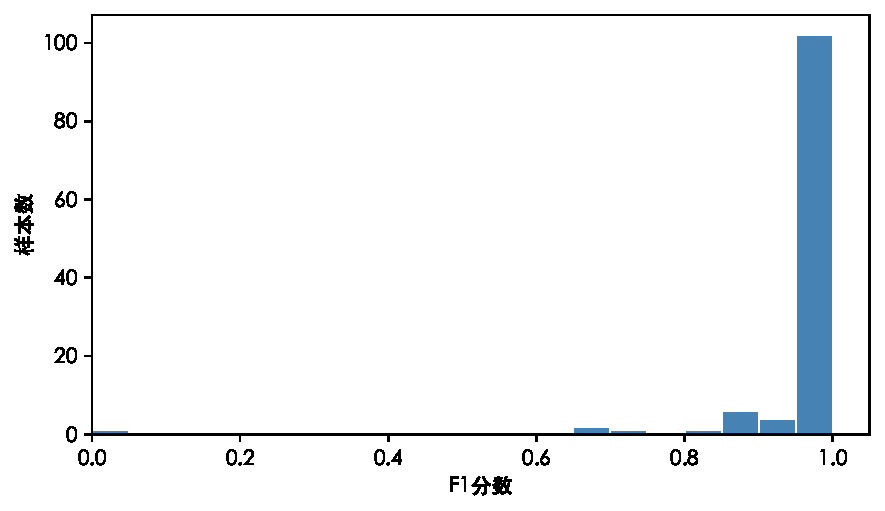
\includegraphics[width=0.75\textwidth]{figures/stage1_f1_dist.pdf}
  \caption{第一阶段测试集F1分数分布}
  \label{fig:stage1-f1}
\end{figure}

分布高度集中于高分区间：73个样本（62.4\%）达到F1=1.0（完全正确），102个样本（87.2\%）的F1$\geq$0.95，106个样本（90.6\%）的F1$\geq$0.9。全部117个样本的平均F1为0.969，平均精确率与平均召回率均为0.969。

\subsection{解析成功样本分析}

仅考虑成功解析的116个样本，平均F1达到0.977，中位数为1.000。73个样本（62.9\%）的F1为1.0，表明模型在这些样本上完整且准确地还原了时序图中所有信号的名称、波形序列与数据标签。F1低于0.95的样本仅有14个（12.1\%），F1低于0.8的样本仅有3个（2.6\%），说明模型在绝大多数样本上的解析质量较高。

图~\ref{fig:good-stage1}展示了一个F1=1.0的复杂样本——一个FIFO读控制器模块的输入时序图。该模块包含14个信号，涵盖时钟与复位信号、7个数据总线信号（共41个数据标签）以及5个二值控制信号，波形中包含密集的数据标签跳变与复杂的控制逻辑交互。模型完整且准确地还原了全部信号的名称、波形序列与数据标签值。

\begin{figure}[htbp]
  \centering
  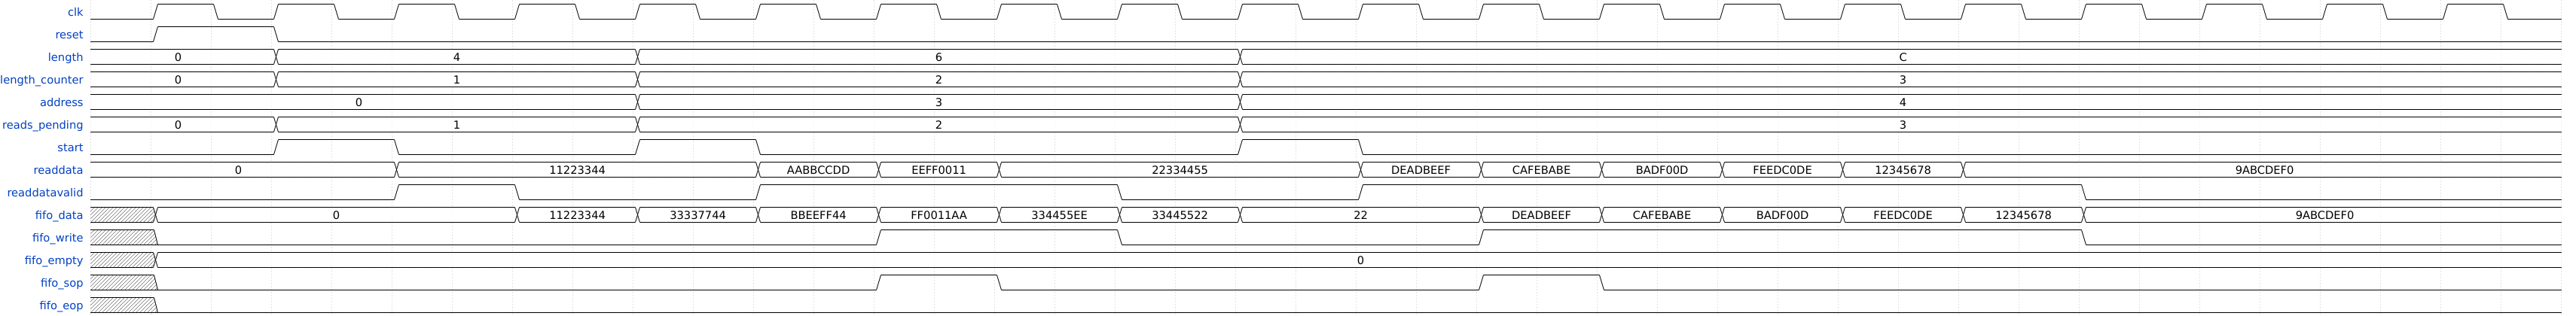
\includegraphics[width=\textwidth]{figures/error_examples/good_stage1.png}
  \caption{第一阶段完全正确的复杂样本：FIFO读控制器模块（14个信号，F1=1.0）}
  \label{fig:good-stage1}
\end{figure}

\subsection{错误模式分析}

对F1低于0.95的14个样本进行信号级对比分析，可归纳出以下两类主要错误模式。

\textbf{波形长度偏差。}最常见的错误类型是模型预测的波形字符串长度与标准答案不一致，即模型对时序图中的时间步总数估计有误。在14个低分样本中，超过半数存在此类问题。

图~\ref{fig:error-wavelen}展示了一个典型案例的输入时序图。该样本为一个纯组合逻辑模块（F1=0.650），包含4个数据总线信号，不含时钟信号。标准答案的波形字符串长度为20，而模型预测的波形字符串长度为40。具体而言，标准答案中每个信号的波形均为连续的数据字符（如\texttt{====================}），表示每个时间步都有新的数据值；而模型在每两个数据字符之间插入了保持符号（如\texttt{=.=.=.=.=.=.=.=.=.=.=.=.=.=.=.=.=.=.=.=.}），将波形长度扩展为两倍。尽管模型正确识别了全部20个数据值及其顺序，但时间步数量的翻倍导致逐步对齐时产生系统性偏移，使F1显著下降。

\begin{figure}[htbp]
  \centering
  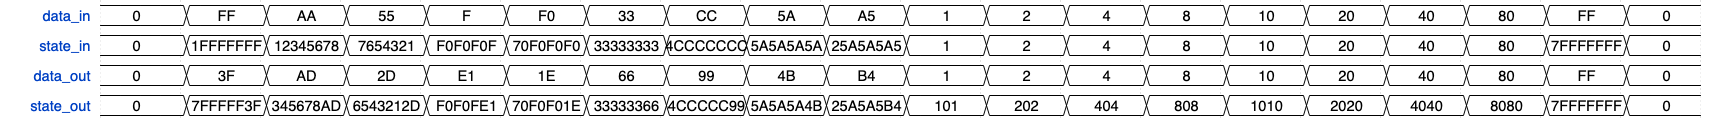
\includegraphics[width=\textwidth]{figures/error_examples/wavelen_gt.png}
  \caption{波形长度偏差示例：纯组合逻辑模块的输入时序图（F1=0.650）}
  \label{fig:error-wavelen}
\end{figure}

如图~\ref{fig:error-wavelen}所示，标准答案（波形长度20）与模型预测（波形长度40）渲染出的时序图在视觉上几乎完全相同——两者包含相同的数据值序列，区别仅在于WaveJSON层面每个数据值是否紧随一个保持符号。正是由于两种波形长度对应的时序图在视觉上无法区分，模型难以从图像中准确判断时间步的总数，从而产生系统性的长度偏差。

\textbf{数据标签识别错误。}部分样本中，模型正确识别了信号名称与波形结构，但数据总线的数值标签存在少量错误。

图~\ref{fig:error-datalabel}展示了一个指令译码器模块（F1=0.887）的前5个信号，其中模型预测中与标准答案不一致的位置以黄色高亮标注。该模块包含13个信号，模型正确识别了全部信号名称与波形的整体结构，但数据标签存在多处错误，且错误分布于多个信号中：寄存器地址输出\texttt{DR}有13处偏差，源操作数地址\texttt{SA}有19处偏差，目标操作数地址\texttt{SB}有13处偏差，立即数输出\texttt{IMM}有25处偏差。从图中可以观察到，错误集中在波形的后半段——前半段的数据标签基本正确，而从中段开始出现局部错位后，后续标签随之发生连锁偏移。这类错误反映了时序图中小字号数值标签的视觉识别难度，尤其当多位数据标签紧密排列时，字符间的区分度降低，单个标签的识别错误会引发后续标签的连锁错位。

\begin{figure}[htbp]
  \centering
  \begin{minipage}{\textwidth}
    \centering
    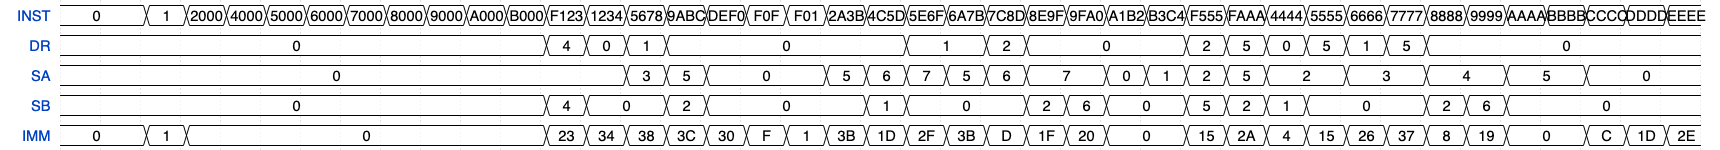
\includegraphics[width=\textwidth]{figures/error_examples/datalabel_gt.png}
    \centerline{（a）标准答案}
  \end{minipage}
  \vspace{0.5em}
  \begin{minipage}{\textwidth}
    \centering
    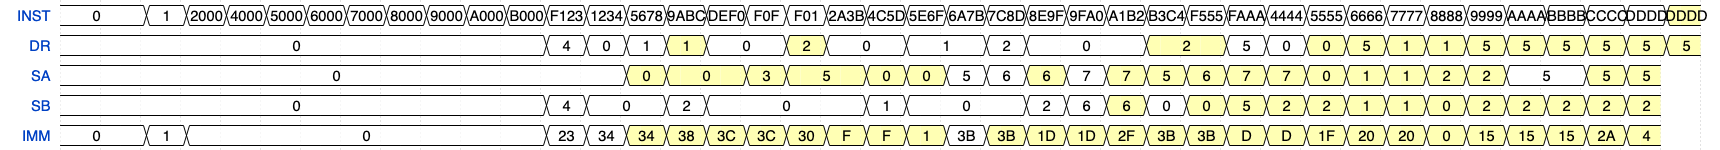
\includegraphics[width=\textwidth]{figures/error_examples/datalabel_pred.png}
    \centerline{（b）模型预测（黄色高亮标注错误的数据标签）}
  \end{minipage}
  \caption{数据标签识别错误示例：指令译码器模块前5个信号（F1=0.887）}
  \label{fig:error-datalabel}
\end{figure}

唯一的解析失败样本是一个包含12个信号的AXI接口模块。模型实际生成了语义正确的WaveJSON内容，但输出的前缀格式异常（在JSON前附加了非预期的文本标签），导致JSON解析器无法提取有效结构。这属于输出格式遵从性的偶发错误，而非模型视觉理解能力的系统性不足。

整体而言，第一阶段模型在时序图到WaveJSON的转换任务上表现优异：信号名称的识别几乎完全正确（所有成功解析的样本均正确识别了全部信号名），波形结构的还原精度高，主要瓶颈在于长时序图的时间步计数精度与密集数据标签的精确识别。


\section{第二阶段实验结果}

本节报告第二阶段（WaveJSON到Verilog代码）有监督微调模型在测试集上的评估结果。评估流程如第~\ref{sec:sim-eval}~小节所述，将模型生成的Verilog模块与对应的测试平台联合仿真，通过波形对拍计算F1分数。测试集共117个样本。

\subsection{总体结果}

为评估微调的效果，本文将微调模型与多个通用大语言模型进行对比，使用相同的测试集与评估流程。基线模型包括微调前的同架构模型Qwen3-8B以及多个大参数量通用模型，均以零样本方式直接推理。为确保对比的公平性，所有基线模型的提示词中均详细说明了任务目标、期望的输出格式（完整的Verilog模块）以及模块接口的约束条件，使模型在不经微调的情况下也能充分理解生成要求。表~\ref{tab:stage2-comparison}汇总了各模型的对比结果。

\begin{table}[htbp]
  \centering
  \caption{第二阶段不同模型的评估结果对比}
  \label{tab:stage2-comparison}
  \begin{tabular}{lcrr}
    \toprule
    模型 & 参数量 & 通过仿真 & 平均F1 \\
    \midrule
    GLM-4.5-Air\inlinecite{glm2025glm45} & 106B (A12B) & 35/117 & 0.253 \\
    DeepSeek V4 Flash\inlinecite{deepseek2025v4} & 284B (A13B) & 40/117 & 0.280 \\
    Qwen3-Coder-480B-A35B\inlinecite{yang2025qwen3coder} & 480B (A35B) & 47/117 & 0.321 \\
    GPT-OSS-120B\inlinecite{openai2025gptoss} & 117B (A5B) & 67/117 & 0.473 \\
    \midrule
    Qwen3-8B\inlinecite{yang2025qwen3} & 8B & 38/117 & 0.263 \\
    Qwen3-8B\inlinecite{yang2025qwen3} + SFT（本文） & 8B & \textbf{79/117} & \textbf{0.614} \\
    \bottomrule
  \end{tabular}
\end{table}

通用模型在零样本设置下的整体F1均低于微调模型。微调前的同架构模型Qwen3-8B的平均F1为0.263，仿真通过率仅32.5\%，与微调后的0.614（67.5\%）形成鲜明对比，表明领域微调显著提升了生成代码的结构规范性与功能正确性。GPT-OSS-120B在基线中表现最优（F1=0.473），其仿真通过率（67/117=57.3\%）也是基线中最高的，但仍低于本文8B参数微调模型。微调模型在仿真通过率与整体F1上均取得了最优结果，且微调后的8B模型超越了参数量高出数十倍的通用模型，进一步验证了领域特定训练的有效性。

在117个测试样本中，79个样本（67.5\%）的生成代码通过了编译与仿真，38个样本（32.5\%）因编译错误或仿真失败未能产出有效波形，F1计为零。各样本的F1分数分布如图~\ref{fig:stage2-f1}所示。

\begin{figure}[htbp]
  \centering
  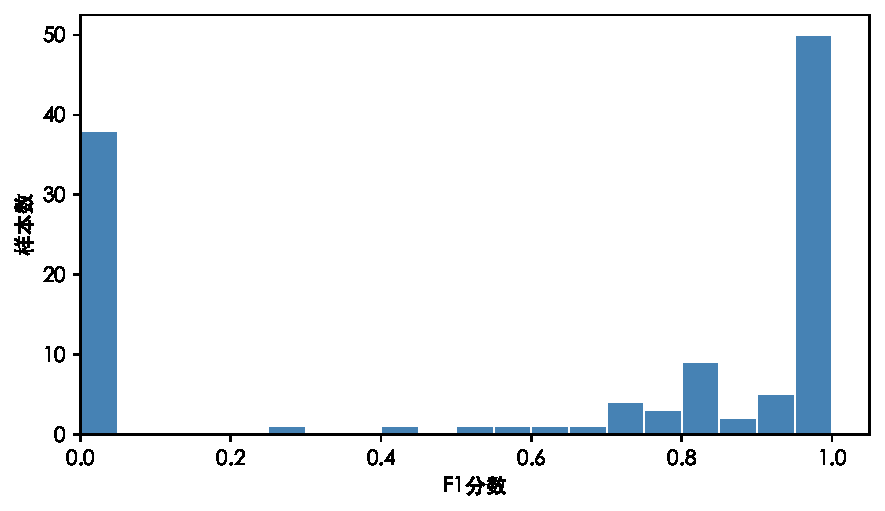
\includegraphics[width=0.75\textwidth]{figures/stage2_f1_dist.pdf}
  \caption{第二阶段测试集F1分数分布}
  \label{fig:stage2-f1}
\end{figure}

分布呈现明显的两极化特征：38个样本集中在F1=0（仿真失败），41个样本达到F1=1.0（完全正确），中间区域的样本相对较少。全部117个样本的平均F1为0.614。

\subsection{仿真成功样本分析}

仅考虑通过仿真的79个样本，平均F1达到0.909，中位数为1.000。其中41个样本（51.9\%）的F1为1.0，表明模型生成的代码在测试平台的全部激励下与标准答案的行为完全一致。F1$\geq$0.8的样本共66个（83.5\%），说明绝大多数成功仿真的样本在功能上高度正确，仅存在局部信号的细微偏差。F1低于0.5的样本仅有2个（2.5\%），表明模型一旦能生成可编译的代码，其功能正确性普遍较高。

图~\ref{fig:good-stage2}展示了一个F1=1.0的复杂样本的输入时序图——一个PCIe QPLL复位状态机控制器。该模块包含15个信号，涵盖时钟锁定检测、DRP配置、PLL复位与上电控制等多个子系统的交互逻辑。模型生成了224行参数化Verilog代码，包含4个模块参数、两级异步寄存器同步链、12状态的有限状态机与5个输出组合逻辑赋值，仿真波形与标准答案完全一致。

\begin{figure}[htbp]
  \centering
  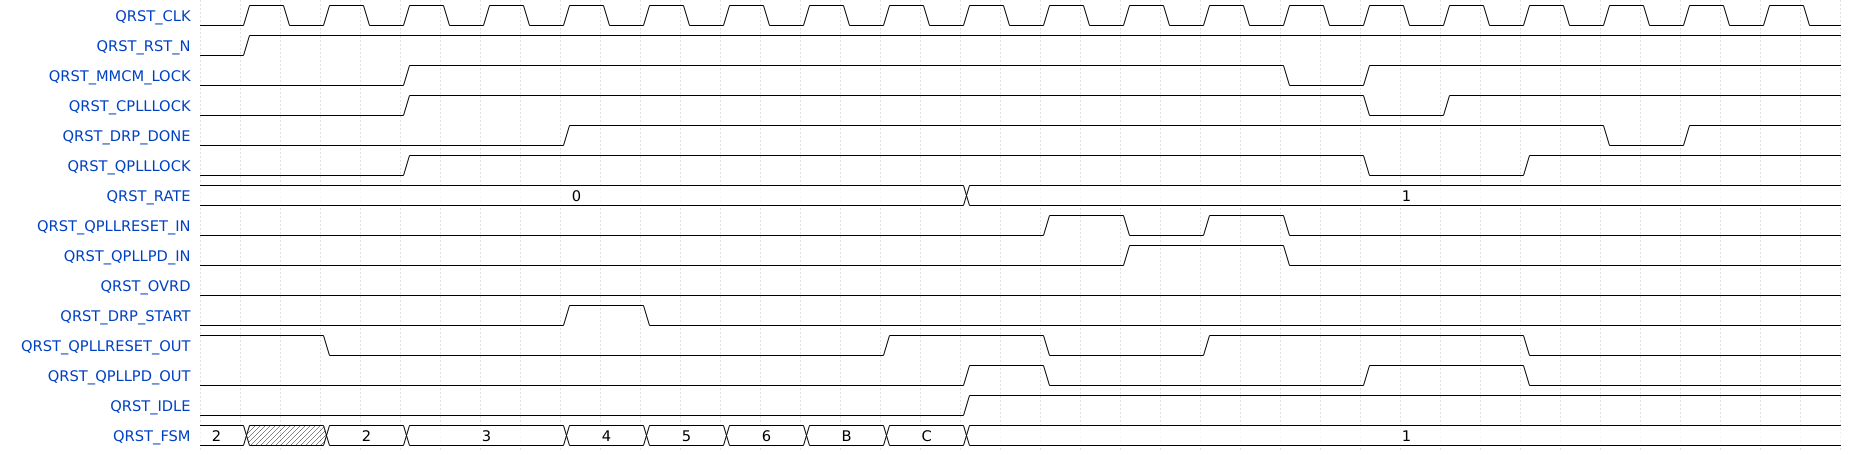
\includegraphics[width=\textwidth]{figures/error_examples/good_stage2.png}
  \caption{第二阶段完全正确的复杂样本：PCIe QPLL复位控制器（15个信号，224行Verilog，F1=1.0）}
  \label{fig:good-stage2}
\end{figure}

\subsection{仿真失败分析}

对38个仿真失败样本的生成代码进行人工分析，按模型能力不足的表现形式可归纳为以下三类。

\textbf{重复退化。}5个样本的生成代码因模型陷入重复生成模式而未能产出有效的模块定义，均缺少完整的\texttt{endmodule}结构。对原始推理输出的逐行分析揭示了四种退化模式：（1）\textit{递增编号的重复声明}——模型声明了状态机框架后，进入形如\texttt{reg ablk\_*\_temp\_N}的临时寄存器声明循环，编号N从1递增至104，1{,}353行输出中有1{,}247行为重复的寄存器声明；（2）\textit{单一词元的无限重复}——模型仅输出模块名的前几个字符后便陷入单个词元的无限复制，32{,}771个字符中仅前29个字符为有意义的代码；（3）\textit{暴力枚举的组合爆炸}——一个14位输入的译码器模块，模型试图逐一列举全部$2^{14}=16{,}384$种输入组合的\texttt{case}分支，在生成583条分支后被截断；（4）\textit{状态机状态爆炸}——一个I\textsuperscript{2}C主控模块被生成为包含244个几乎相同状态的巨型状态机，每个状态仅执行简单的计数等待后跳转至下一状态，完全偏离了协议的实际逻辑。这类错误的共性在于模型未能形成对模块整体结构的规划，在生成过程中陷入局部模式的机械重复，直至达到词元上限。

\textbf{端口接口错误。}部分样本的生成代码虽然结构完整，但端口声明与测试平台的期望不匹配，导致联合编译失败。典型的错误模式包括：遗漏测试平台所需的模块参数（如数据位宽参数\texttt{DATA\_WIDTH}、地址位宽参数\texttt{ADDR\_WIDTH}等）、输出端口位宽与测试平台声明不一致（如测试平台期望16位输出但模型生成了24位端口）。这类错误表明模型在从WaveJSON推断模块接口规格时存在偏差，尤其在参数化模块的参数列表还原方面能力不足。

\textbf{逻辑实现错误。}部分样本的生成代码能够通过编译甚至完成仿真，但内部逻辑实现存在缺陷，导致仿真波形与标准答案产生偏差。这是有监督微调模型最具代表性的错误类型：模型从训练数据中学会了Verilog代码的结构模式——端口声明、\texttt{always}块框架、\texttt{case}语句骨架——但仅凭词元级交叉熵损失的监督，难以精确还原决定功能行为的关键细节。

对38个通过仿真但F1$<$1.0的样本进行信号级分析，发现10个样本存在输出信号退化为常量的现象——标准答案中随输入变化的输出信号在生成代码的仿真中始终保持固定值。以下三个典型案例展示了这类错误从组合逻辑到时序逻辑、从控制信号到数据通路的多种表现形式。

\textit{组合逻辑译码失效。}一个指令译码器模块（F1=0.407）的13个端口中，输入信号\texttt{INST}被正确传递，但12个译码输出中大部分始终保持零值或未定义态。标准答案中，寄存器地址字段\texttt{DR}、\texttt{SA}、\texttt{SB}应从指令中提取不同位段，控制信号\texttt{MB}、\texttt{LD}、\texttt{MW}应根据指令类型产生使能脉冲。模型生成的译码器包含了正确的\texttt{case}语句框架，但译码条件与输出赋值的对应关系存在大量错误，导致绝大多数指令未能命中有效分支。

\textit{时序逻辑状态机停滞。}一个行扫描控制器（F1=0.584）的15个信号中，4个输入信号被正确复现，但11个输出中有5个始终为高阻态，其余在复位释放后恒为零。标准答案显示该状态机应循环执行行加载序列——\texttt{prev\_row\_load}、\texttt{curr\_row\_load}、\texttt{next\_row\_load}依次以一个周期的偏移产生使能脉冲。模型生成的代码包含了状态寄存器与转移逻辑的框架，但转移条件不完整，状态机无法离开初始状态。

\textit{数值映射偏差。}一个相位译码器（F1=0.254，通过仿真的样本中最低分）的输入信号被正确复现，但4个相位输出的数据标签值与标准答案显著不同。例如，\texttt{dqs\_phase}的标准标签序列为\texttt{16}、\texttt{36}、\texttt{56}、\texttt{77}、\texttt{7}、\texttt{27}、\texttt{48}、\texttt{68}，反映相位值随输入地址的查表映射关系，而模型生成的序列为\texttt{66}、\texttt{25}的简单交替。模型能够还原信号的跳变时序，但无法准确推断具体的数值映射。

上述三类错误呈现出一致的模式：模型在代码框架层面基本正确——端口结构、控制流骨架、信号类型均能从WaveJSON中正确识别，但在决定功能行为的关键细节——译码真值表的具体条目、状态转移的精确条件、数值映射的查找表——上存在系统性偏差。需要指出的是，评估采用相同测试平台的仿真对拍，模型只需生成在该激励下行为一致的任意实现即可获得满分，并不要求与标准答案的代码相同。模型未能找到任何一个功能等价的实现，反映的是模型从行为观测推断逻辑规则的能力不足。

这一错误模式具有重要的方法论启示。有监督微调的词元级损失函数对功能正确性的监督是间接的——它优化的是生成序列与参考代码之间的词元匹配度，而非生成代码的功能行为。上述案例表明，词元级匹配能够引导模型学会代码的结构模式，但不足以保证行为层面的正确性。同时，这类错误产生的部分正确输出——F1分布在0.25至0.58之间，而非全零——恰好为基于仿真奖励的强化学习提供了有意义的优化梯度。第~\ref{chap:method}~章提出的GRPO方法正是针对这一瓶颈：以仿真对拍的F1分数作为连续值奖励信号，直接在功能正确性层面优化模型，下一节将报告其实验结果。


\section{强化学习实验结果}

本节报告在SFT检查点基础上进行GRPO强化学习训练后的评估结果。训练共进行230步，评估流程与第二阶段SFT模型相同。

\subsection{总体结果}

表~\ref{tab:stage2-rl}对比了SFT模型与GRPO模型在测试集上的表现。

\begin{table}[htbp]
  \centering
  \caption{GRPO强化学习优化前后的评估结果对比}
  \label{tab:stage2-rl}
  \begin{tabular}{lrrr}
    \toprule
    模型 & 通过仿真 & 平均F1 & 仿真成功F1 \\
    \midrule
    Qwen3-8B + SFT & 79/117 & 0.614 & 0.909 \\
    Qwen3-8B + SFT + GRPO & \textbf{89/117} & \textbf{0.630} & 0.828 \\
    \bottomrule
  \end{tabular}
\end{table}

GRPO训练将仿真通过率从67.5\%（79/117）提升至76.1\%（89/117），净增10个样本能够通过编译与仿真，整体平均F1从0.614提升至0.630。这一结果表明，基于仿真奖励的强化学习能够在SFT基线之上继续改善生成代码的编译正确性。

\subsection{结果分析}

对比SFT与GRPO的结果，可以观察到以下特点：

\textbf{编译通过率的提升。}GRPO模型的仿真通过数从79个增至89个，净增10个样本。具体而言，19个SFT阶段编译失败的样本在GRPO后成功通过仿真，同时有9个SFT阶段通过仿真的样本在GRPO后出现了编译错误。仿真失败的28个样本中，18个因编译失败、10个因语法错误被排除。与SFT模型的38个失败样本相比，GRPO训练有效减少了生成代码中的语法与结构性错误，说明仿真奖励引导模型学会了更规范的代码生成模式。

\textbf{仿真成功样本的F1变化。}仅考虑通过仿真的样本，SFT模型的平均F1为0.909，而GRPO模型为0.828。这一下降的原因在于：GRPO新增通过仿真的19个样本大多为SFT阶段完全失败（F1=0）的困难样本，虽然现在能够通过编译，但功能正确性尚未达到高水平，拉低了仿真成功子集的平均分。整体F1仍然从0.614提升至0.630，表明新增样本的贡献超过了个体F1的下降。

\textbf{优化方向的验证。}230步的GRPO训练将整体F1从0.614提升至0.630，主要贡献来自将更多样本从“完全失败”转化为“部分正确”。这一结果验证了基于仿真奖励的强化学习作为SFT后续优化手段的可行性，同时也表明在有限的训练步数下，模型的优化主要体现在代码结构规范性的改善上，功能逻辑层面的深层优化仍需更充分的训练。

\subsection{典型改善案例}

为直观展示GRPO训练的具体改善效果，本节列举三个SFT模型编译失败但GRPO模型成功生成可仿真代码的典型样本。

\textbf{案例一：超声发射脉冲控制器（F1：$0 \to 0.951$）。}该模块包含6个信号，输入包括时钟、接收门控、发射延迟参数与脉宽参数，输出为差分发射脉冲对TXP/TXN。SFT模型生成了121行的单块代码，声明了20余个寄存器与10个\texttt{parameter}常量，试图实现一个包含5个状态的发射控制有限状态机，但其中引用了未声明的变量（如\texttt{PulseCtrNext}），导致编译失败。GRPO模型生成了22行简洁代码，虽然逻辑实现为简化的门控赋值而非完整状态机，但端口声明规范、语法正确，仿真波形与标准答案的F1达到0.951。

\textbf{案例二：存储器仲裁状态机（F1：$0 \to 0.936$）。}该模块为一个包含13个信号的存储器访问仲裁器，需要在CRT显示请求、CPU读请求与CPU写请求之间进行优先级调度。SFT模型生成的代码结构完整——包含正确的状态定义、状态转移逻辑与组合输出——但将三个输出端口（\texttt{crt\_gnt}、\texttt{cpu\_wr\_gnt}、\texttt{cpu\_rd\_gnt}）声明为\texttt{output reg}后又使用\texttt{assign}连续赋值驱动，违反了Verilog语法规则（\texttt{reg}类型不能被\texttt{assign}驱动），导致编译失败。GRPO模型将输出逻辑改为在\texttt{always}块中以时序逻辑赋值，避免了类型冲突，成功通过编译与仿真。

\textbf{案例三：处理器程序计数器（F1：$0 \to 0.854$）。}该模块是一个包含13个信号的处理器PC单元，涉及分支目标缓冲（BTB）、返回地址栈（RAS）、流水线停顿控制等多个子系统的交互。其输入包括\texttt{btb\_target}、\texttt{ras\_target}、\texttt{good\_target}等32位地址信号以及\texttt{pc\_go}、\texttt{stall}等控制信号，输出为\texttt{pc\_out}与\texttt{pc\_plus4}两个地址序列。SFT模型生成的代码因端口声明与类型定义的不一致导致编译失败；GRPO模型生成了34行代码，正确实现了PC的多路选择与递增逻辑，仿真波形在13个信号中大部分与标准答案一致。

上述案例呈现出一致的改善模式：SFT模型在复杂模块上倾向于生成过度复杂的代码——更多的寄存器声明、更多的状态定义、更多的中间变量——但这些复杂结构中往往包含类型冲突或未声明变量等结构性错误。GRPO训练通过仿真奖励引导模型学会了“可编译优先”的生成策略：倾向于生成结构更简洁、类型声明更规范的代码，即使逻辑上有所简化，也优先确保代码能够通过编译并产出仿真结果。这一策略偏移直接反映了仿真奖励函数的设计——编译失败的代码获得零奖励，而任何能够通过仿真的代码即使F1不高也能获得正奖励，使模型在探索过程中逐步学会避免结构性错误。
